\begin{figure*}[t]
\centering
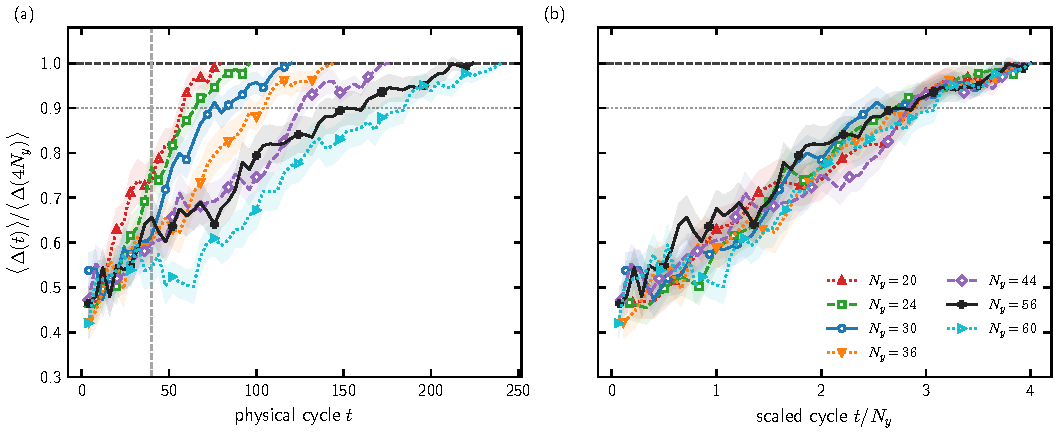
\includegraphics[width=\textwidth]{gap_convergence_size_comparison.pdf}
\caption{Finite-time gap convergence across circumferences.
Hard-wall slab-only purification at $N_x=20$, with $S=100$ independent Born
trajectories per size, maximally mixed slab initialization and Born-conditioned
exterior preparation, through $4N_y$ cycles.
The minimum absolute modular energy is taken within each trajectory,
divided by $2t$, and then averaged.
The ratio of ensemble means
$\langle\Delta(t)\rangle/\langle\Delta(4N_y)\rangle$ is shown against
(a) physical cycle and (b) scaled cycle.
Bands are ordinary sampling SEMs propagated with the within-trajectory
covariance between numerator and reference; no bootstrap or fit is used.
The dashed and dotted horizontal lines mark unity and $0.9$;
the vertical line in (a) marks $t=40$.
The $4N_y$ value is a finite-time reference, not an assumed asymptotic gap;
the common endpoint at unity is imposed by normalization.
These data are distinct from the full-measurement protocol.}
\label{fig:gap-convergence-size-comparison}
\end{figure*}
